\documentclass[border=3pt]{standalone}
% Preâmbulo compartilhado pelos diagramas TikZ da aula 7 de IHR (Emoção)
\usepackage[T1]{fontenc}
\usepackage[utf8]{inputenc}
\usepackage{lmodern}
\usepackage{amsmath}
\usepackage{xcolor}
\usepackage{tikz}
\usetikzlibrary{arrows.meta,angles,quotes,decorations.pathmorphing,decorations.pathreplacing,calc,
                positioning,shapes.geometric,shapes.misc,backgrounds,fit,
                math}

% Paleta (mesma dos SVGs originais)
% Paleta da disciplina de IHR: acento azul (#1A6FB5), cor de destaque do tema.
% (o nome "dblue" é mantido para não alterar todos os diagramas)
\definecolor{dblue}{HTML}{1A6FB5}
\definecolor{dorange}{HTML}{B3541E}
\definecolor{dgreen}{HTML}{4A7C59}
\definecolor{dred}{HTML}{9C4B4B}
\definecolor{dcream}{HTML}{F4F1EA}
\definecolor{dshade}{HTML}{DDD7C9}

% Função gaussiana (não normalizada por padrão de escala visual)
\pgfmathdeclarefunction{gauss}{3}{%
  \pgfmathparse{1/(#3*sqrt(2*pi))*exp(-((#1-#2)^2)/(2*#3^2))}%
}

% Estilos comuns (prefixo d... para não colidir com chaves internas do pgf)
\tikzset{
  >={Stealth[length=2mm]},
  dguide/.style={gray!55, dashed, line width=0.4pt},
  daxis/.style={gray!60, line width=0.7pt, ->},
  dbody/.style={fill=black!3, draw=black!80, line width=1pt},
  dacc/.style={draw=dblue, line width=1pt},
  dlbl/.style={black!55, font=\small},
  dsub/.style={black!45, font=\footnotesize},
  dstate/.style={circle, draw=black!80, fill=dcream, line width=1pt,
                 minimum size=17mm, font=\large, inner sep=1pt},
  dobs/.style={circle, draw=black!80, fill=dshade, line width=1pt,
               minimum size=14mm, font=\large, inner sep=1pt},
  dbox/.style={rounded corners=2pt, draw=black!80, fill=dcream, line width=1pt,
               align=center, inner sep=6pt},
  dop/.style={circle, draw=black!80, fill=white, line width=1pt,
              minimum size=6mm, inner sep=0pt, font=\small},
  dtrans/.style={->, dblue, line width=1pt},
  dmeas/.style={->, dorange, line width=1pt},
  dcurve/.style={line width=1pt, dblue},
  dcurveb/.style={line width=1.4pt, dorange},
}

\begin{document}
\hyphenpenalty=10000 \exhyphenpenalty=10000 \tolerance=9999 \emergencystretch=3em
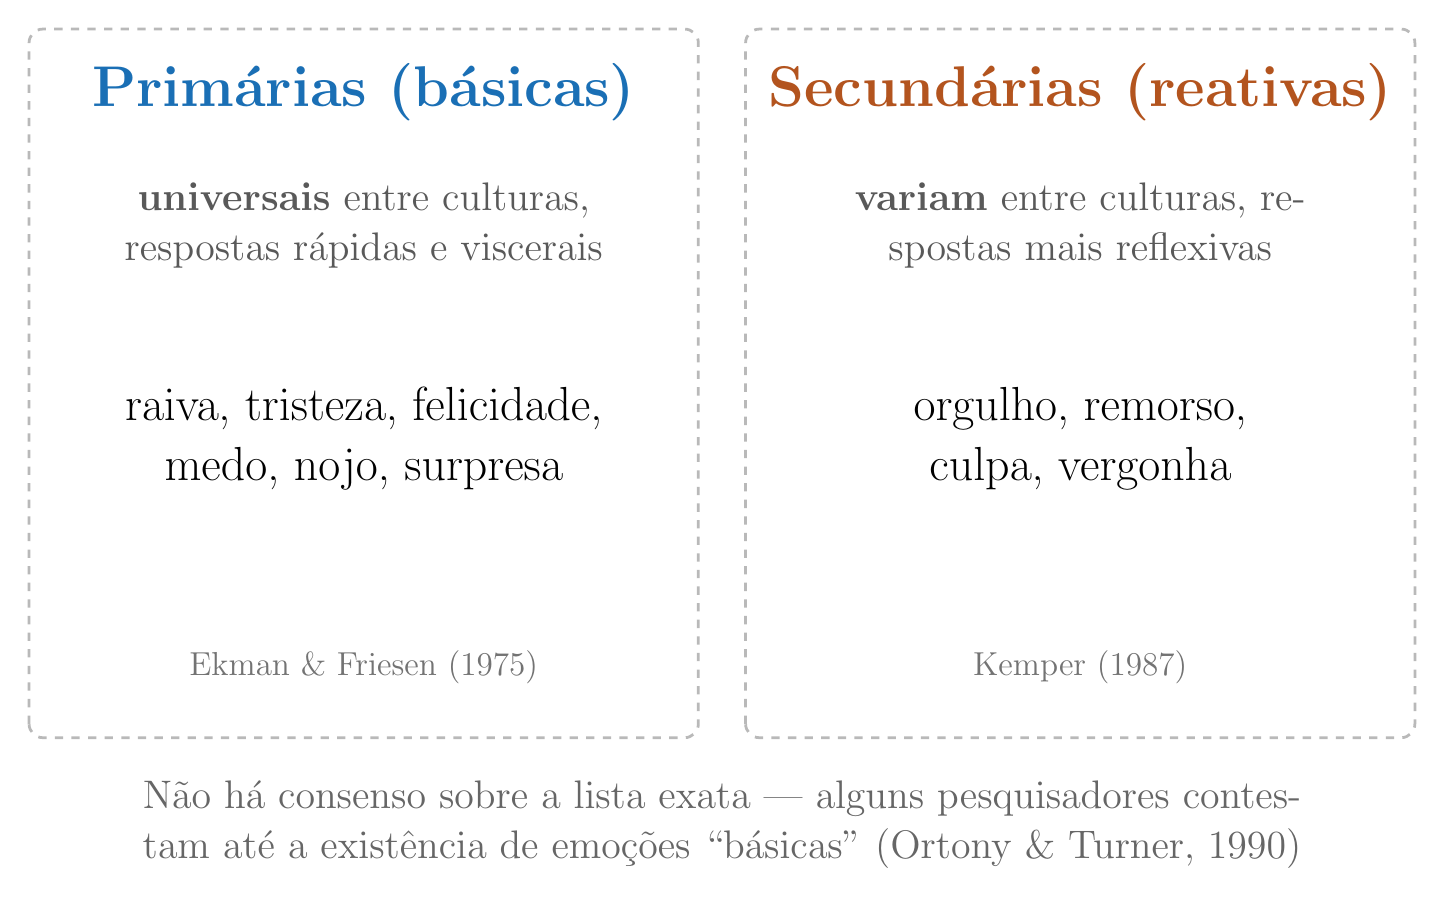
\begin{tikzpicture}[x=1cm,y=1cm]

  % Primárias
  \draw[dguide, rounded corners=5pt, line width=1pt, fill=white] (-8.8,-4.6) rectangle (-0.3,4.4);
  \node[font=\huge\bfseries, dblue] at (-4.55,3.6) {Primárias (básicas)};
  \node[font=\Large, black!65, align=center, text width=7.6cm] at (-4.55,1.9)
     {\textbf{universais} entre culturas, respostas rápidas e viscerais};
  \node[font=\LARGE, align=center, text width=7.6cm] at (-4.55,-0.8)
     {raiva, tristeza, felicidade, medo, nojo, surpresa};
  \node[font=\large, black!55, align=center] at (-4.55,-3.7) {Ekman \& Friesen (1975)};

  % Secundárias
  \draw[dguide, rounded corners=5pt, line width=1pt, fill=white] (0.3,-4.6) rectangle (8.8,4.4);
  \node[font=\huge\bfseries, dorange] at (4.55,3.6) {Secundárias (reativas)};
  \node[font=\Large, black!65, align=center, text width=7.6cm] at (4.55,1.9)
     {\textbf{variam} entre culturas, respostas mais reflexivas};
  \node[font=\LARGE, align=center, text width=7.6cm] at (4.55,-0.8)
     {orgulho, remorso, culpa, vergonha};
  \node[font=\large, black!55, align=center] at (4.55,-3.7) {Kemper (1987)};

  \node[font=\Large, black!60, align=center, text width=17cm] at (0,-5.7)
     {Não há consenso sobre a lista exata --- alguns pesquisadores contestam até a existência de emoções ``básicas'' (Ortony \& Turner, 1990)};

\end{tikzpicture}
\end{document}
